%%========================================================================
%% LaTeX sjabloon voor stage/projectrapport of bachelorproef
%%  HoGent Bedrijf en Organisatie
%%========================================================================

%%========================================================================
%% Preamble
%%========================================================================

\documentclass[pdftex,a4paper,12pt,twoside]{report}

% XXX: Let op: dit sjabloon is gemaakt om dubbelzijdig af te drukken
% Voor enkelzijdig, verwijder ``twoside'' hierboven.

%%---------- Extra functionaliteit ---------------------------------------

\usepackage[utf8]{inputenc}  % Accenten gebruiken in tekst (vb. é ipv \'e)
\usepackage{amsfonts}        % AMS math packages: extra wiskundige
\usepackage{amsmath}         %   symbolen (o.a. getallen-
\usepackage{amssymb}         %   verzamelingen N, R, Z, Q, etc.)
\usepackage[english]{babel}    % Taalinstellingen: woordsplitsingen,
                             %  commando's voor speciale karakters
                             %  ("english" voor EN)
\usepackage{eurosym}         % Euro-symbool €
\usepackage{geometry}
\usepackage{graphicx}        % Invoegen van tekeningen
\usepackage[hyphens]{url}
\usepackage[pdftex,bookmarks=true,breaklinks]{hyperref}
                             % PDF krijgt klikbare links & verwijzingen,
                             %  inhoudstafel
                             
\renewcommand{\UrlBreaks}{\do\/\do\a\do\b\do\c\do\d\do\e\do\f\do\g\do\h\do\i\do\j\do\k\do\l\do\m\do\n\do\o\do\p\do\q\do\r\do\s\do\t\do\u\do\v\do\w\do\x\do\y\do\z\do\A\do\B\do\C\do\D\do\E\do\F\do\G\do\H\do\I\do\J\do\K\do\L\do\M\do\N\do\O\do\P\do\Q\do\R\do\S\do\T\do\U\do\V\do\W\do\X\do\Y\do\Z}

\usepackage{listings}        % Broncode mooi opmaken
\usepackage{multirow}        % Tekst over verschillende cellen in tabellen
\usepackage{rotating}        % Tabellen en figuren roteren
\usepackage{natbib}          % Betere bibliografiestijlen
\usepackage{fancyhdr}        % Pagina-opmaak met hoofd- en voettekst

\usepackage[T1]{fontenc}     % Ivm lettertypes
\usepackage{lmodern}
\usepackage{textcomp}

\usepackage{pgfplots}

\usepackage{lipsum}          % Voor vultekst (lorem ipsum)

%%---------- Layout ------------------------------------------------------

\pgfplotsset{width=7cm,compat=1.13}

% hoofdingen, enz.
\pagestyle{fancy}
% enkel hoofdstuktitel in hoofding, geen sectietitel (vermijd overlap)
\renewcommand{\sectionmark}[1]{}

% lijn, wordt gebruikt in titelpagina
\newcommand{\HRule}{\rule{\linewidth}{0.5mm}}

% Create a graph for the average runtime of an insert, update or delete operation
\newcommand{\CUDGraph}[2]{
\begin{tikzpicture}
\begin{axis}[title=#1, xlabel={Cache ratio}, ylabel={Avg runtime (ns)}, ymin=0, ymax=5000]
\addplot table {#2};
\end{axis}
\end{tikzpicture}
}

% Leeg blad
\newcommand{\emptypage}{
\newpage
\thispagestyle{empty}
\mbox{}
\newpage
}

% Gebruik een schreefloos lettertype ipv het "oubollig" uitziende
% Computer Modern
\renewcommand{\familydefault}{\sfdefault}

% Commando voor invoegen Java-broncodebestanden (dank aan Niels Corneille)
% Gebruik: \codefragment{source/MijnKlasse.java}{Uitleg bij de code}
\newcommand{\codefragment}[2]{ \lstset{%
  language=java,
  breaklines=true,
  float=th,
  caption={#2},
  basicstyle=\scriptsize,
  frame=single,
  extendedchars=\true
}
\lstinputlisting{#1}}

%%---------- Documenteigenschappen ---------------------------------------
%% Vul dit aan met je eigen info:

% Je eigen naam
\newcommand{\student}{Frederik De Smedt}

% De naam van je lector, begeleider, promotor
\newcommand{\promotor}{Joeri Van Herreweghe}

% De naam van je co-promotor
\newcommand{\copromotor}{Jens Buysse}

% Indien je bachelorproef in opdracht van een bedrijf of organisatie
% geschreven is, geef je hier de naam.
\newcommand{\instelling}{---}

% De titel van het rapport/bachelorproef
\newcommand{\titel}{Research of caching strategies in mobile native applications using external data services}

% Datum van indienen
\newcommand{\datum}{29 mei 2015}

% Faculteit
\newcommand{\faculteit}{Faculty Business \& Information Management}

% Soort rapport
\newcommand{\rapporttype}{Bachelor's thesis submitted to achieve the degree of\\Bachelor in the Applied Computer Science}

% Academiejaar
\newcommand{\academiejaar}{2015-2016}

% Examenperiode
%  - 1e semester = 1e examenperiode
%  - 2e semester = 2e examenperiode
%  - tweede zit = 3e examenperiode
\newcommand{\examenperiode}{Examination period 2}

%%========================================================================
%% Inhoud document
%%========================================================================

\begin{document}

%%---------- Front matter ------------------------------------------------
%% Het voorblad - Hier moet je in principe niets wijzigen.

\begin{titlepage}
  \newgeometry{top=2cm,bottom=1.5cm,left=1.5cm,right=1.5cm}
  \begin{center}

    \begingroup
    \rmfamily
    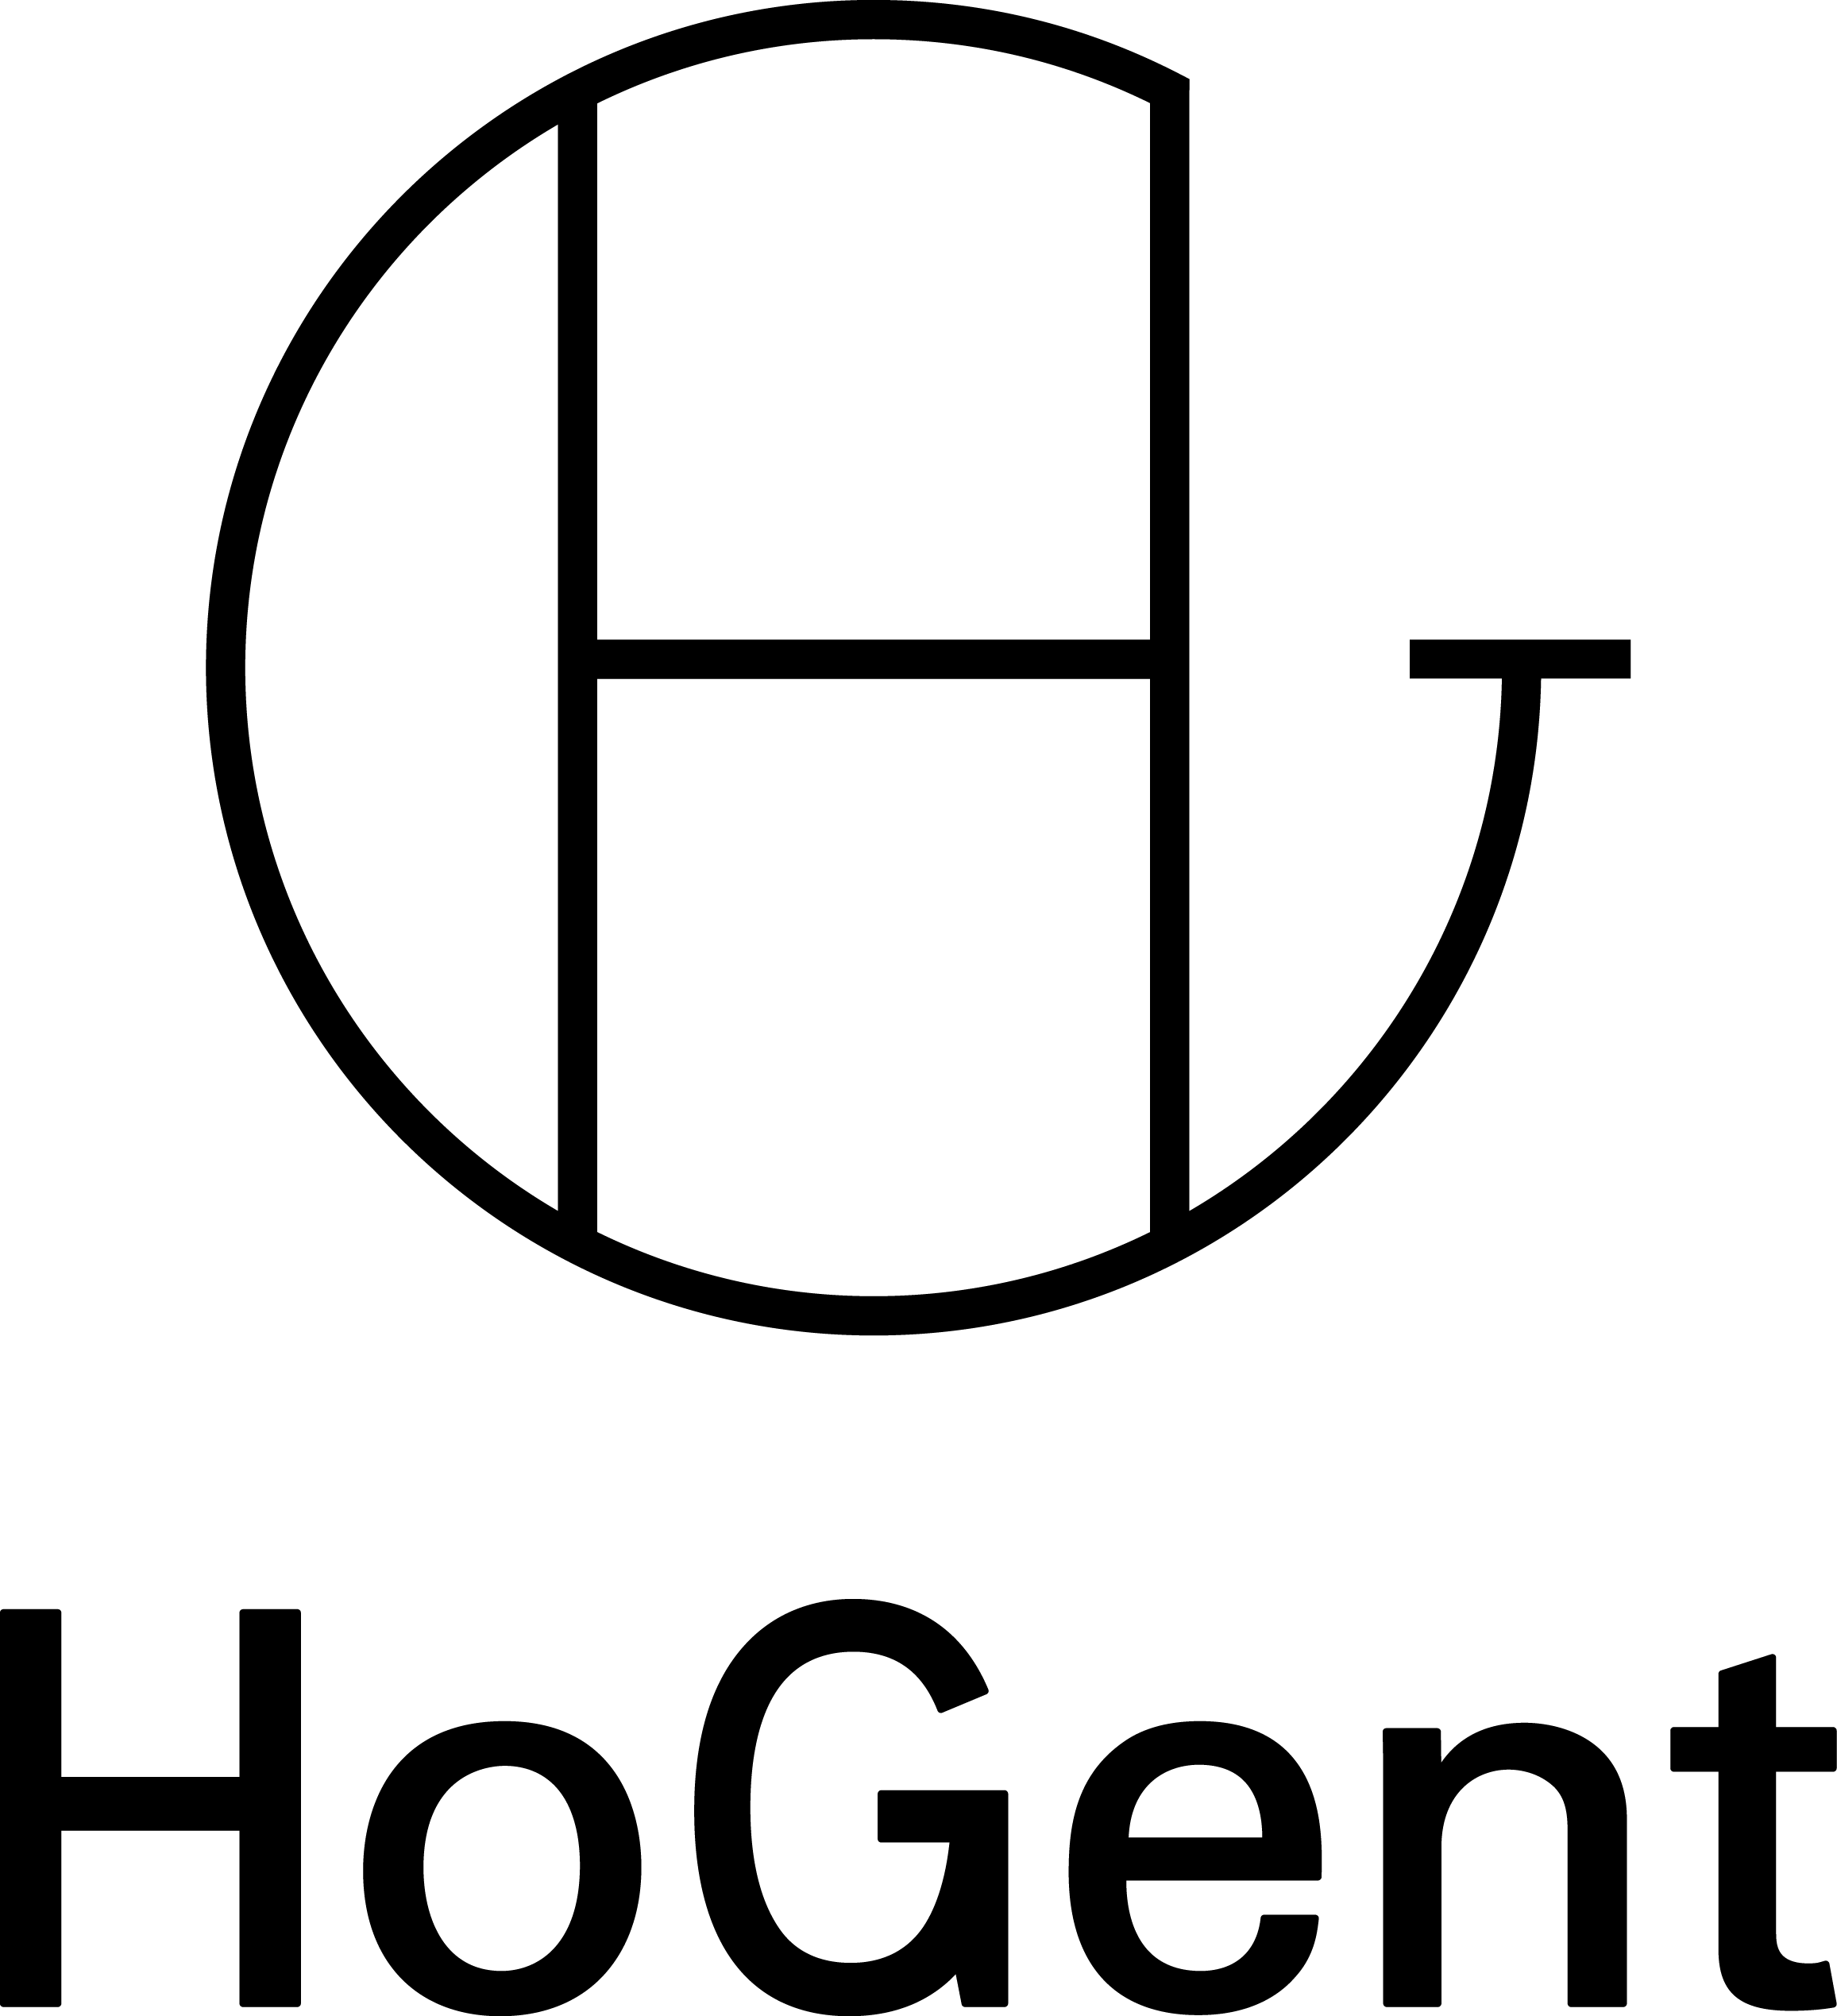
\includegraphics[width=2.5cm]{img/HG-beeldmerk-woordmerk}\\[.5cm]
    \faculteit\\[3cm]
    \titel
    \vfill
    \student\\[3.5cm]
    \rapporttype\\[2cm]
    Promotor:\\
    \promotor\\
    Copromotor:\\
    \copromotor\\[2.5cm]
    Organisation: \instelling\\[.5cm]
    Academic year: \academiejaar\\[.5cm]
    \examenperiode
    \endgroup

  \end{center}
  \restoregeometry
\end{titlepage}

% Schutblad

\emptypage


\begin{titlepage}
  \newgeometry{top=5.35cm,bottom=1.5cm,left=1.5cm,right=1.5cm}
  \begin{center}

    \begingroup
    \rmfamily
    \faculteit\\[3cm]
    \titel
    \vfill
    \student\\[3.5cm]
    \rapporttype\\[2cm]
    Promotor:\\
    \promotor\\
    Copromotor:\\
    \copromotor\\[2.5cm]
    Organisation: \instelling\\[.5cm]
    Academic year: \academiejaar\\[.5cm]
    \examenperiode
    \endgroup

  \end{center}
  \restoregeometry
\end{titlepage}

\begin{abstract}
When discussing caching, one might think about large, optimized systems like servers or very low-level systems where efficiency is the main priority, like processors, yet regular-sized can be easily forgotten. In this paper the usages of a cache in mobile applications are discovered and is divided in three research questions. The main research question is what cache replacement algorithms can be used in a mobile application to provide efficient caching. To answer this question, several performant and popular cache replacement algorithms are discussed and are then benchmarked in an Android application. These results are then collected and analysed to decide which of the cache replacement algorithms is the best. Next is dicussed how this cache can be synchronized with the backend, to make sure that the objects used on the client are not too outdated. This will be solely based on research and uses the knowledge of the first question to understand how and why some of these techniques can be used. Based on possible lifecycle events that can occur in mobile applications, synchronisation and cache management might have to adapt. Several noticeable lifecycle events will be considered from the most popular mobile platforms: Android, iOS and Windows (Phone). These two parts make the last chapter of this thesis.
\end{abstract}

\chapter*{Preface}
\label{ch:voorwoord}
As the final part of my education at the College of Ghent, I had to write a thesis of a specific subject relevant to the domain I am studying: Applied Computer Science.
I have been confronted with the power of caching before, in both bigger applications and mobile apps, so I was already familiar with the basics of caching. APIs using caches in mobile apps do, however, each have their own way of caching. This made me curious in the research that had been done to objectively determine the performance of caches in mobile applications. Yet I found no real research that really focussed on verifying the performance of caches on mobile devices, it was for this reason I decided to choose this subject as the subject of my thesis.
\\\\
I would like to thank my promotor Joeri Van Herreweghe and my copromotor Jens Buysse, for reviewing my work and for supporting me and the subject of this thesis. I would also like to thank my parents and sister for understanding and encouraging me and my education for all these years.
\\\\
It is recommended that the reader understands the basic concepts of programming. If the reader would like to really understand the code written to create the benchmark results used in this thesis, he/she should have decent knowledge of Java and basic knowledge of Android.

\tableofcontents

% Als je een lijst van afkortingen of termen wil toevoegen, dan hoort die
% hier thuis. Gebruik bijvoorbeeld de ``glossaries'' package.

%%---------- Kern --------------------------------------------------------

\chapter{Introduction}
\label{ch:introduction}
The definition of mobile has changed a lot in the last few years and the expectations of mobile applications continue to rise.
Mobile applications should work on a myriad of devices and screen resolutions, and should take battery efficiency into account.
Furthermore is an application no longer really considered mobile if it isn't available without a stable internet connection.
This makes research about caching in mobile applications really interesting since it can solve multiple problems.
Caching of the results of expensive operations, e.g. an internet connection, will allow the system to avoid many of these operations,
reducing battery consumption, and can these results be used when a (temporary) connection loss would occur.
\\\\
Lots of IT companies already implement such a system:
\begin{itemize}
\item The Facebook-app still shows several posts and pictures when the user has no internet connection.
\item Third-party API's, such as Picasso (Android) and SDWebImage (iOS) retrieve images from the web and have an embedded caching system.
\item Twitter allows the user to change account settings offline, which are later synchronized with the backend when a connection is established\footnotemark.
\end{itemize}
\footnotetext{This is more about persistent data, however it is used to store temporary data that can later be forgotten once it is synchronized with the backend. Just like a cache containing business data.}
\newpage
\section{Problem definition and research questions}
However mobile caching is becoming more and more common, there is no real framework on which they all rely. Instead they each have to think about how to implement
caching and have to invest in discovering caching strategies and inventing a good caching implementation.
\\\\
They can decide to ignore the caching problem and focus on the business logic and the actual functional requirements of the project. The chances that the
project is able to be completed within the deadline increases, as they have less work to do. However, if there is a non-functional requirement that requires some sort of caching
or if the users of the application are complaining about problems that come along (e.g. lots of traffic or battery usage), one would have to implement the caching system afterwards. Which might force the developers to redesign parts of the system (both frontend and backend) or forces them to do this in an incomplete way, introducing lots of bugs that usually come along in caching systems.
\label{sec:research questions}
Every platform already has some infrastructure designed to allow caching, e.g. Guava and a local lightweight database.
Yet there is more to caching than simply storing information, developers should think about what data is eligible for caching and how this can improve their application.
They should be able to do this with an efficient method, customized to the needs of the application considering all possible events that might occur and how they might be able to handle this. These ideas and strategies should then be implemented in both the backend and frontend, however the backend implementation could be reduced to an almost non-existing implementation, since it is not merely about the native application itself, but about the data flow between the different systems.
\\\\Because of these reasons, the following questions will be answered in this article:
\begin{itemize}
\item How can a caching strategy efficiently store and fetch data in a native mobile application?
\item How can the cache be updated or changed based on lifecycle events in mobile applications?
\item How can the cache be synchronized with the external data service (backend)?
\end{itemize}
\chapter{Methodology}
\label{ch:methodology}
First, a literature study has taken place about caching in general: what concepts and principles are used? Which steps can be differentiated when interacting with a cache? What are some common techniques? Some of these were later revisited to test them on a mobile device.
\\\\
All these concepts and ideas are then tested in a case study, which will analyze the performance of a frontend Android application. The performance measurements are created by running benchmarks on several cache replacement algorithms with several different traces.
\\\\
After the case study, the events that are commonly handled by a mobile native application are discussed and how they fit in with the bigger picture concerning caches. However the case study will be performed in the Android platform, it is important to consider all platforms (Android, iOS, Windows) and how each of them handles these events.
\\\\
Last, a literature study concerning the synchronization between the frontend cache and the underlying data service was done. Although some part can be partially out of the scope of the frontend developer, it is important that everyone has a clear view of what they can do to facilitate synchronization. The backend can influence frontend performance and the frontend can influence backend performance.
\chapter{Basics of caching}
\label{ch:caching}
A cache can be defined as a (fast) memory structure designed to reduce costs and improve speeds of computer operations.
The term caching is widely used in computer science, from the CPU that uses different multi-level caches, to web caches concerning
the reuse of already fetched HTTP pages \citep{rfc2616} and all of them are designed to improve performance. Even low-end devices such as microcontrollers
can benefit on the usage of a cache \citep{extremetech_multilevelcache}. How this memory structure improves the performance
is dependent on the use case in which it used. It could keep the results of long operations or use tokens to check whether data is outdated.
\section{Basic cache performance metrics}
The presence of a cache by itself will not cause a performance increase. It is integrated in a software application that uses a cache. The application then checks whether certain data is present in the cache and if not, does everything it needs to do in order to retrieve this data from a third party. In most examples a cache can be represented by a collection of key/value pairs, to which the application requests a value based on a key. When the cache contains the data the application is requesting, it is commonly known as a \emph{cache hit}. Inversely, when the cache does not contain the requested data, it is known as a \emph{cache miss}. The relationship between the total amount of requests and the total amount of hits is the \emph{hit ratio}.
$R=h/n$ where $R$ is the hit ratio, $h$ is the total amount of cache hits and $n$ is the amount of cache requests.
These terms are, among others, important factors determining the performance of a cache. A common misconception is that a high hit ratio results in better cache performance, yet this is only true considering hit ratios. If the hit ratio were the only factor, the caches ``performance'' would be proportional to the size of the cache and a cache of 10Tb always yield better performance than a cache of 20Mb \citep{wulf1995hitting}. This statement can easily be proven wrong when considering other factors such as speed, as the 20Mb cache will need far less time to produce a result than the cache of 10Tb.
\section{Paging}
However caching is of high importance with lots of aspects in IT, caching is what it is today thanks to some specific problems that have received lots of attentions the last decades. Perhaps the most important problem, considering the field of caching, is the problem with \emph{virtual memory} \citep{denning1970virtual}. Virtual memory maps virtual memory addresses, provided by an operating system to a program, to actual hardware memory addresses. This way, the operating system can manage its memory resources and decide where to store and retrieve data from programs using virtual memory. This was considered a very elegant way to increase programming productivity, as programmers could use a high-level API to retrieve and store data instead of needing to talk directly to the processor, which would also make them machine dependent.
\\\\
The operating system can assign priorities to memory addresses and decide whether it should be stored on a fast or slow memory. The memory of an idle process could for example be persisted on slow memory, i.e. hard drive, so that the faster memory, i.e. RAM, can be used for memory of currently active processes. The moment that the idle process wakes up, it can still use the virtual memory pointers, as if the data has never moved. When a process tries to access a piece of data, currently stored on the hard drive, the operating system will produce a \emph{page fault}. This event will cause the \emph{page}, a block of data, containing the desired data on the hard drive to be transfered to somewhere in RAM memory.
\\\\
The memory transfer due to a page fault is however very expensive as the hard drive is a lot slower than RAM memory and the processor itself. Therefore it is important to have a good paging strategy, an algorithm that decides which pages will be persisted to the hard drive and which pages will remain in RAM memory. The optimal algorithm will only persist the pages that will not be used for the longest period of time.
\\\\
The paging problem is very similar to finding the optimal caching strategy, RAM memory is the cache, the hard drive is non-cached memory and developers and researchers are looking for an algorithm such that only the least interesting memory is removed from the cache. The principle ultimately solving the paging problem is therefore one of the fundamental principles not only in pages and virtual memory, but all of caching, this principle is called the \emph{locality principle}.
\\\\
\section{Locality principle}
\subsection{What is the locality principle}
When people are executing a process, such as preparing dinner, they always tend to gather everything they need before or during the process. If it were a bigger meal the entire meal is divided in a set of subprocesses. When preparing lasagne it could be divided in preparing the tomato sauce, creating each layer using previously prepared ingredients, etc. The principle of dividing a large task in a set of smaller subtasks is called \emph{divide and conquer}. % TODO: Find reference for divide and conquer
When creating the lasagne layers, one would first collect all supplies needed (tomato sauce, lasagne sheets, etc) and put them somewhere close, e.g. on the counter, once that is done, the layers are assembled. This is more practical and time saving than to continually walk a relatively long distance each time the tomato sauce is needed.
\\\\
Something similar has been discovered with programs by \cite{locality_principle} when analyzing memory usage of multiprogramming systems using virtual memory in 1967.
He formalized this idea through the years and called it the \emph{locality principle} also commonly known as \emph{locality of reference}. He found that programs intrinsically use a very small part of data when performing arbitrary algorithms. In 1980 he formally defined a relationship between the processor, executing the instructions, and the data/object it uses called the \emph{distance} and is denoted as $D(x,t)$ where x is the object and t is the current time. The relevance of this object to the processor at a certain time is based on whether the distance is less than a certain threshold:
\[
	D(x,t) \leq T
\]
where T is the threshold and D(x,t) is the distance function. The threshold and the distance are embedded in a, usually 2 dimensional, spatial-temporal coordinate space where the spatial dimension is the memory address of the object and the temporal dimension is the time when it was accessed.

\subsection{Interpreting spatial-temporal distances}
Because the distance function $D$ is operating in a spatial-temporal space, it is based on the definition and interpretation of the two different dimensions.
The easiest way to understand how these dimensions can be interpreted is to look at them seperately. Once that is understood, there should be a function
$m : S \times T \to \Theta$ where $S$ is the set representing the spatial dimension, $T$ is the set representing the temporal dimension and $\Theta$ is the set representing the spatial-temporal space.
\newpage
\emph{Temporal distance}, the distance in time that can be expressed in several ways:
\begin{itemize}
\item time since last reference
\item time until next reference
\item access time to get the object
\item a combination of the above or others
\end{itemize}
The time since the last reference to object $x$ can be known by storing the references used by the processor and the time when the reference happened in a list. The time until next reference might yield better results when trying to create an effective and efficient cache since it is known when the object will be used again. However this should require a learning agent that can try and calculate when the next reference will happen based on the reference history. The time unit used should be a relative unit such as the execution of an instruction, this is better than an absolute unit such as seconds because it will ignore external factors that shouldn't affect the distance, e.g. other processes running.
\\\\
\emph{Spatial distance}, the distance to the location of the object can be expressed in several ways as well:
\begin{itemize}
\item the amount of hops in a network required to retrieve the contents
\item the memory on which the data is stored, e.g. objects stored in RAM have a smaller spatial distance than objects stored on a hard drive
\item the number of memory addresses between the object and the addresses currently being used or pointed to
\item a combination of the above or others
\end{itemize}
Intuitively, one could see a relationship between the spatial and temporal locality. When the spatial distance to an object is greater, the temporal distance usually also increases because it will need to cover more ground to retrieve the object. When the temporal distance is greater the spatial distance will usually increase because of pacification of the object: it will be stored on slower memory due to the lack of interaction.
When checking the relevance of objects to the processor are checked, with $D(x,t) \leq T$, only some objects will pass the inequality, the set of these objects is 
called the \emph{working set}. It are the objects in the working set that would, among others, be candidates for caching. 
\section{CRUD}
When interacting with a cache, there are, in general, several operations that each cache is able to do. In general, one would want all operations that allow the developer to read the contents of a cache and to get from an arbitrary cache state, to any other arbitrary cache state through, possibly composite, operations. These operations are known as CRUD operations and are a main part of RESTful web services \citep{battle2008bridging}. This will allow an easier implementation when using Read Through (or Cache Aside) Caches.
% TODO: Add reference to section about read through and cache aside
\emph{CRUD} is an acronym for Create Read Update Delete and as the name suggests, 4 operations can be distinguished:
\begin{itemize}
\item \emph{Create} allows some client to add an object to a data set. When adding an object to a cache this will typically invoke an add-function receiving two arguments: a key and a value. SQL implements this with its INSERT-statements and HTTP integrates this using a POST request.
\item \emph{Read} is used to get all information or a subset of information from a data set, in a typical cache this will be integrated as a get-function receiving
the key of the value one would wish to access. \emph{The key passed to the function is the same key that is passed to the add-function when creating a new cache entry.} SQL implements this with its SELECT-statements, commonly known as queries, and HTTP integrates this using a GET request.
\item \emph{Update} will change the contents of an existing object, this is separated from Create as these two might be treated differently, depending on the system in which the data set is embedded. A cache will mostly provide a common API for both Create and Update: a function with a key and a value as its parameters. Yet they might be seperated into separate functions to increase readability or to simplify event triggering. SQL implements this with its UPDATE-statement and HTTP implements this using PUT-requests.
\item \emph{Delete} is used when an element should no longer be an element of the data set. In a cache this might happen when an object is outdated, or if the object has also been removed in the data service. One would then call a delete-function passing the key of the object that should be removed. SQL implements this with its DELETE-statements and HTTP integrates this with its DELETE request.
\end{itemize}
\citep{battle2008bridging} Note how these operations are defined on the database-level, software application level, and networking level. Also note how an interface of a cache should at least contain functions allowing the user to execute all CRUD-operations, yet they are not limited by them.
\chapter{Cache replacement algorithms}
\label{chap:caching_algorithms}
With a concrete list of \emph{what} should be possible with caches, one can discuss \emph{how} this could all be implemented, the algorithms implementing a cache system are called \emph{cache replacement algorithms} or \emph{cache replacement policies}. Yet not just any cache replacement algorithm will do, it is an art to find the most optimal algorithm, the one that will provide the best (performance) results by interacting with it using CRUD-operations.
Although most algorithms are only based on CRUD interactions with the cache, some algorithms can be run on separate processes/threads that are
then responsible for maintaining the cache even without interactions with the user.
\section{RR}
The first cache replacement algorithm that will be discussed is the Random Replacement strategy. Of all the strategies, this one could be considered one of the strategies with the lowest overhead and the easiest implementations \citep{random_replacement}. This makes it ideal for certain low-level systems or hardware that cannot afford many processing cycles on cache management.
\paragraph{Read} When trying to get a certain object by its key, the algorithm can use any sorted or non-sorted collection. When using an non-sorted collection it would check each element in the collection in $\mathcal{O}(n)$. Note how this defines the upper bound of the function, therefore it could also be in constant time or $\mathcal{O}(\log_2n)$ when performing a binary search on a sorted list.
\paragraph{Create} When adding an object while the cache is not yet full, it could simply be added to the collection, algorithm-independently. When the cache is already full, the algorithm will randomly remove replace an object from the collection by the new object that should be stored. The operation itself is primitive and easy to program, the only difficulty is creating a reliable random generator, yet this is not in the scope of this algorithm.
\paragraph{Update} Updating is similar to \emph{create}, if the key is present it will result in a \emph{read} to get the appropriate object and then changes the object. If the key is not in the cache, it could either \emph{create} object or alarm the user that it is not present.
\paragraph{Delete} When deleting an object, based on a key, it can be done by first performing a \emph{read} to know whether the key is present and if so removing it. Yet some collections will do this nevertheless, in that scenario the algorithm could simply delegate to the delete function from the backing collection.
\section{FIFO}
FIFO, acronym for First-In-First-Out, is a cache replacement policy much like a queue. New objects are inserted at one end of the queue, when the cache is full the first object at the other end will be discarded and the new object will be added at the insertion end \citep{reineke2007timing}. FIFO is analogous to FCFS, First-Come First-Served, which is used in OS scheduling algorithms.
Note that the hit ratio performance of the FIFO replacement strategy is like the hit ratio performance of the RR replacement strategy \citep{rao1978performance}.
\paragraph{Read} A read in a FIFO policy results in a queue being scanned in $\Theta(n)$, almost just like RR. The difference between RR and FIFO is that a FIFO cannot be a sorted collection, since its performance is based on a ``constantly'' defined sorting structure, this means that one cannot just swap two elements in the cache and expect it to work just the same: the actual state of the cache has changed. Just like RR, a read does not change the state of the cache.
\paragraph{Create} When adding a new object to the cache it will, without loss of generality, be placed on the left side of the queue. When the queue is full, the first element on the right will be removed and all other objects will be ``moved to the right'' (however this is not an actual operation that occurs in an efficient queue implementation), clearing a space on the left, ready to be filled in by the new object.
\paragraph{Update} When updating an existing object, based on a key, there will be a read that will then change the object at the index $i$ by the new object. After the object $x$ is updated, $x$ should then be removed from the queue, every element left of $x$ should then be moved to the right and $x$ is again added to the left side of the queue. Note that all these operations should be executed in a procedural or atomic way.
\paragraph{Delete} When deleting an existing object, the algorithm scans the queue until it finds the index with value $x$ corresponding to the given key. It will then remove $x$ and move all elements left of $x$ to the right. The next object added to the queue will therefore not cause the object (completely) at the right to be removed from the cache.
\section{CLOCK}
This cache replacement algorithm produces similar results as the FIFO implementation described above, yet it uses a different internal algorithm to accomplish these results. It uses a circular collection, which repeats from the start when trying to retrieve the element after the last element. Using a queue this could be implemented by linking the next pointer of the last element to the first element \citep{clock_cpan}. Using an array one can always a modulus operator based on the size of the array to have get an index that is always lower than the size of the cache. At any given time there will be an index pointing to the ``current'' item, this is used throughout the text as the index pointer or $R$, using an array this can be an integer, using a linked list this can be an entry holding a value and references to the next and previous elements.
\paragraph{Read} Linearly scans the cache starting at $R$, scan ends when $R$ is the same as when the operation started or if the key is found. If the key is found, the key will be registered as being referenced, which could be a boolean or integer.
\paragraph{Create} If the cache is full, check whether the element at $R$ is referenced, if not replace the element with the new element and increment $R$, otherwise increment $R$ and repeat this operation. Worst case scenario, every element was initially referenced. In this scenario after having added the new element, every element will not be referenced and the element at the initial $R$ will be replaced. If the cache is not yet full, add the element before the element at $R$ (in a linked list this will be in $\mathcal{O}(1)$) and do not change $R$. This allows the cache to always stay in a consistent FIFO state, as the cache can, at any point remove or read the cache in the correct order.
\paragraph{Update} Find the element, update its value, signify it is not being referenced and increment $R$ to point to the next element. If the element is not yet in the cache, this is the same as a create operation.
\paragraph{Delete} The element is read in the cache and removed and the size of the cache is decremented. When using a linked list, the algorithm will, indirectly, connect the previous element and next element to each other. When using an array one would need to pull every element after $R$ to the left, decrementing their indexes. This means that the linked list implementation runs in $\mathcal{O}(1)$ while the array implementation runs in $\mathcal{O}(n)$.
\section{LRU}
An \emph{LRU}-cache (Least Recently Used Cache). There are lots of variants on LRU and therefore it can also be seen as a cache replacement algorithm family. The probability of an object being present in a cache, the hit rate $h(n)$, can be approximated by 
$h(n) \approx 1 - e^{-q(n)t_C}$, where $n$ is the object being requested, $q(n)$ is the popularity of the object (see \emph{Zipf's law}) and $t_C$ being the (unique) root of 
$\sum_{n=1}^N(1-e^{-q(n)t})=C$, with $N$ being the maximum amount of objects in the cache and $C$ the cache capacity. This approximation is called the \emph{Che approximation} \citep{fricker2012versatile}.
\\\\
The LRU algorithm is all about replacing the least recently used object, in other words, when a new object should be added to a full cache, it will remove the object that hasn't been accessed for the longest period of time. To know when an object has last been accessed, the usual implementation uses a map, let's call it the \emph{key history map} that can get a timestamp (this can be in milliseconds or can be some relative time unit) based on a key. However it could also be implemented by a queue, where the order of the queue determines which objects have, relatively, been accessed most recently.
\paragraph{Read} Retrieving an object based on a key, first boils down to retrieving a value from any collection, just like RR. When the object is found it will not immediately return this, yet it will firstly access the \emph{key history map} and update the timestamp to its newest value. This way the algorithm will know, in the future, that this key has just been accessed. If the LRU is implemented using a queue, it will, without loss of generality, remove the object $x$ at index $i$, (conceptually) move all objects left of $i$ to the right (which is equivalent to incrementing the index $j$ of all objects where $j < i$) and $x$ will then be inserted at the left side of the queue.
\paragraph{Create} If the cache is not yet full, the object will be added to the collection and the key history map will be updated with a new timestamp for the specified key. If the cache is full, it will first find the key with the lowest timestamp, which is the object that hasn't been accessed for the longest period of time (considering an increasing time function). It will then remove this key in the collection and remove the corresponding key from the map, the object will then be added to the collection and the key history map will be updated with a new timestamp for the specified key. When using a queue with a cache that is not yet full, one would add the new object, without loss of generality, to the left side of the queue. When using a queue with a full cache, one will remove the object to the right of the queue, move all remaining objects to the right, and then add the new object to the left of the queue.
\paragraph{Update} The algorithm will check if the key is already stored in the collection, if not, this boils down to \emph{creating} (adding) a new object to the collection or queue. When the key is stored in the cache, it will update the object in the collection to the new object and then it will update the timestamp of the corresponding key in the key history map. When using a queue, it will remove the object with the specified key from the queue, move all objects to the left of the object to the right, and then add the new object, without loss of generality, to the left side of the queue.
\paragraph{Delete} To remove an object from the cache, the object is simply removed from both the collection and the key history map. When using a queue, it will remove the object $x$ from the queue and move all objects left of $x$ to the right.
\\\\
\citep{lru_implementation}This is the basic implementation of an LRU cache, yet there are lots of variants. There are algorithms taking a new approach, based on LRU, there are some algorithms that have a highly specialized implementation of LRU, and there are even some implementations that use LRU together with some other cache replacement algorithm to try and get optimal results based on the situation it is in.
\section{MRU}
The next algorithm is very similar to LRU, \emph{MRU} is an acronym for \emph{Most Recently Used} and will evict the most recently accessed objects when adding a new object to an already full cache. LRU and MRU should not be seen as ``competitors'' of each other, but rather a twin where, most of the time, one of the two can be chosen based on the context.
If it makes sense that a recently requested object has a high probability of being requested again in the near future, LRU might be a good choice. If it makes more sense that a recently requested object will not be requested any time soon, an MRU cache replacement strategy might be better. Even though one would think LRU would be used most of the time, there are abundant scenario's where MRU would make a lot of sense also. Consider a cache containing Facebook-posts, would it work better under an MRU or an LRU system? To answer this question further research should be done, but MRU makes a very good candidate, considering people tend not to revisit posts they have just visited 10 minutes earlier. If the user were to respond or like the post, he could however receive notifications of new people posting comments and thus LRU could be more useful.
\paragraph{Read} Every object in the cache stores an extra bit (or boolean) called the MRU-bit and is used to find out whether the object has recently been visited, let's
say that every object in the cache is stored as a tupel $(b,x)$, where $b$ is the MRU-bit and $x$ is the actual object stored. First the algorithm will check if the object is present in the cache and if so, this will be the index $i$ and it will set $b$ to 1 or true. This is used to indicate that it has just been accessed. Next the algorithm will check if there exists another index where the MRU-bit is not 1, if so the algorithm ends, otherwise it will flip the MRU-bit at every index back to 0 or false, this is called a 
\emph{global-flip}. This is the same as checking if $\exists i \in I : B(i) = 0$, where $I$ is the collection of all indexes and $B : I \to \{0,1\}$ is the function that gets the MRU-bit of the object at an index. This can be refactored as $\forall i \in I : B(i) = 1$, so checking for the existence of an index with an MRU-bit at 0 or false is the same as checking whether every MRU-bit is 1 or true.
\paragraph{Create} When the cache is not yet full, the next object will be added to the end of the cache and its MRU-bit will directly be set to 1 or true (ensuring it will not 
be replaced before the next \emph{global-flip}. If the cache is full it will look for an index $j$, such that $B(j) = 0$ and $\forall i \in I : i < j, B(i) = 0$, so $j$ is the first index with a 0 or false MRU-bit. Note that there will \emph{always} be at least 1 index with a 0 or false MRU-bit due to global-flipping.
\paragraph{Update} If the object is not yet present in the cache, it will delegate the object to \emph{create}. If it is in the cache, it will replace the object, while keeping it at the same position, and set its MRU-bit to 1 or true. If the MRU-bit was previously 0 or false, it is important to check if a \emph{global-flip} should be executed or not. Yet it is always safe to check for this, even if the MRU-bit hasn't changed (and already was on 1 or true).
\paragraph{Delete} To remove an object, the algorithm first checks whether the object is present in the cache, if it is not then it doesn't have to do anything, if it is present at index $i$, it moves the object at every index $j$ such that $j > i$ to the left which is the same as decrementing $j$ by one, so $j \leftarrow j - 1$.
\\\\
\citep{guan2014wcet} Having discussed the basic MRU and LRU algorithms one can now respond to temporal localities with different characteristics.
\section{LFU}
\label{sec:LFU}
LFU, acronym for Least Frequently Used, is a cache replacement algorithm that looks at how many times an object is accessed. This means that the object that has been accessed the least will be evicted when adding a new object to an already full cache. Just like MRU and LRU, this cache is only benefitial in specific scenario's.
\\\\
When creating a cache for a web server, static pages, images, css-files, etc. are stored in a cache. This cache will then be accessed with every request to check for its presence, before retrieving the file from some other slower source. One might think LRU is a good idea since the most popular, and therefore the most requested, objects will be present in the cache. This is true to some extent, yet only in some concrete scenario's. Imagine that the ``GET /index.html'' HTTP request would call $n$ different objects in the cache. If the LRU-cache were to have a maximum size limit $N$ such that $N < n$, the cache will be adding new elements to the cache to later remove it during the same request. This is where LFU might be more meaningful, even with a maximum size limit $N < n$. The LFU algorithm will give a better ranking to common objects that would be accessed over lots of different request, say a logo or common CSS file.
\\\\
There are several implementations of an LFU cache, yet the algorithm from \cite{shah20101} will be discussed, which ensures $\mathcal{O}(1)$.
This implementation uses two data structures, (1) a hashmap where an element can be accessed in $\mathcal{O}(1)$, this is possible if the hash function used is an 
\emph{injective} function with an upper limit $u$. It could then map each hash to a single array index of an array of size $u$ which can obviously be stored, retrieved, removed and updated in $\mathcal{O}(1)$. (2) A frequency list, which is a bidirectional linked list that contains an element having a number marking its frequency and having another bidirectional linked list of all cache objects. These cache objects each hold a reference to the frequency element they are in.
\paragraph{Read} The hashmap is used to retrieve the cache object based on a key. It will then use its reference to get the frequency element it is in, and use the frequency list to, without loss of generality, traverse to the next element on the right, which should be the next ordered frequency node. If the object were already referenced once, therefore it would be in the 1-node, it would then go to the 2-node. If this node does not exist, it will create it and add it to the right of the current frequency node and to the left of the next frequency node. Now that the cache object is under the next frequency node, the algorithm will check whether the previous frequency node still contains cache objects, if not it will remove the frequency node from the frequency list. Note that however there are particularly more steps than some other algorithms, it is still in $\mathcal{O}(1)$.
\paragraph{Create} When the cache is not yet full, it will add the object to the first node of the frequency list, which is the 1-node signifying the object has been referenced once, and will possibly create this node if it is not yet present. If the cache is already full, the first frequency node will be taken (mostly yet not limited to the 1-node) and from there will take any of the linked cache objects and remove if from the linked list and from the hashmap. After this it can just add the object as the cache is no longer full.
\paragraph{Update} To update an object, the algorithm will get the cache object, based on its key, from the hashmap and then update the contents of the cache object. After this it will get the frequency node, with frequency number $n$, based on its reference, go to the $(n+1)$-node (which is possibly created if it does not yet exist), and adds it to its linked list. If the object does not exist in the cache it could either throw an appropriate exception or delegate to the \emph{create} procedure.
\paragraph{Delete} To remove an object from the cache, the algorithm will first retrieve the object from the hashmap, based on the key. It will then remove itself from the linked list from the frequency node it is in, possibly removing the frequency node if there are no more elements in it. And last but not least it will remove the object from the hashmap based on the key.
\\\\
Note how the constant execution time of the algorithm fully depends on the hashmap implementation used. If it is an implementation such as described above, it will provide a constant execution time, yet if it were $\mathcal{O}(\log n)$ or $\mathcal{O}(n)$, the algorithm would no longer have the constant execution time.
\section{LIRS}
\emph{LIRS}, \emph{Low Inter-reference Recency Set Replacement Policy} \citep{jiang2002lirs}, is a cache replacement algorithm based on LRU. 
The major performance problem with LRU is that it always assumes that the object that has been referenced the least recent is the one that will not be accessed for the longest period of time. Yet in some (even trivial) cases, this is simply not the case: imagine a relational database with a B-tree for efficiently retrieving $N$ indexes for a set of $N$ records where there exists a bijective function from an index to a record. In the cache blocks of data are stored with a fixed-size where an index is made up of $I$ blocks and a record is made up of $R$ blocks, therefore there are $I \cdot N$ index blocks and $R \cdot N$ record blocks, where $I < R$. Because every operation on a record will first find the record based on the index B-tree, the probability of an index block being accessed will be higher than the probability of a record block being accessed. Yet in a simple LRU-cache it will most of the time favor record blocks in its cache as those are the last referenced blocks in a typical database operation. A cache favoring index blocks would however be more efficient as it increases the cache hit ratio. \emph{LIRS} tries to solve such a problem by looking at its IRR, \emph{Inter-Reference Recency}, which is the amount of referenced blocks between the last and second-to-last reference of a certain block. Say there exist objects $A$, $B$ and $C$ the following reference history could exist:
\[ABCBABCCBCABC\]
The initial \emph{IRR} of $A$ is 3 (with $BCB$ in between) and the next is 5 (with $BCCBC$ in between). When adding a new object to the cache $A$ will be the first object to be replaced because it has the highest \emph{IRR}. In a cache implementationt there is a set of objects with a low IRR (\emph{LIR}) and a set of objects with a high IRR (\emph{HIR}), the cache mainly exists of \emph{LIR} objects, which are never considered for replacement. A small subset of the cache's memory is used for \emph{HIR} objects, that are eligible for replacement. When an \emph{HIR} object has a lower IRR than some \emph{LIR} object, the two will be swaped and the \emph{LIR} object becomes an \emph{HIR} object and the \emph{HIR} object becomes an \emph{LIR} object.
\\\\
An LIRS cache consists of a data structure called a \emph{LIRS stack}, which contains two queues: one used for LIR objects (\emph{LIR stack}), of size $L_{lirs}$ and one used solely for HIR objects (\emph{HIR stack}), of size $L_{hirs}$. In general $L_{lirs} \gg L_{hirs}$, where $L_{hirs}$ could even be only $1\%$ of $L_{lirs}$. The object on top of each queue is the most recent accessed object and the bottom object is the least recently accessed object, similar to an \emph{LRU stack}.
Stack pruning, which is commonly used in the CRUD operations, is the removal of HIR objects from the bottom of the stack until a LIR object is present at the bottom.
\\\\
Every object in the LIRS stack is either a LIR or a HIR object, if it is a LIR object, it will always be fully accessible in the LIRS stack and will not be (completely) removed when adding a new object. Every HIR object is either a \emph{resident HIR object} or a \emph{non-resident HIR object}. A HIR object is resident if it is present in the HIR stack, otherwise --- if it is only present in the LIR stack --- it will be non-resident.
\paragraph{Read} When referencing an HIR object it will be added to the top of the LIR stack, removing the bottom element of the corresponding stack and a stack prune will be conducted. If the HIR object was already in the LIR stack it is promoted to an LIR object and its reference in the HIR stack is removed. If the HIR object wasn't yet present in the LIR stack its reference is placed on top of the HIR stack, yet there shouldn't be any object removed from the HIR stack as there is no new item that was added. If the object is a non-resident HIR object, it will still promote to a LIR object, yet nothing will need to be done on the HIR stack as it wasn't present in that stack, by definition. If the object is not yet in the cache, this results in a create operation.
\paragraph{Create} When adding a non-existing object to a partially filled LIRS cache, the object will be added to the top of the LIR stack and to the top of the HIR stack. If the LIR stack is already full, the object will be added to the HIR stack, possibly removing the least recent (bottom) object from the stack if it was already full. Note how the removed HIR object could still have a reference in the LIR stack, which would now be a non-resident HIR object.
\paragraph{Update} When changing an existing object in the cache it will be the same as a read operation where the underlying value is changed. It is imperative that this is not simply a delete-create operation, as the replacement policy would then forget this objects history.
\paragraph{Delete} When deleting a resident HIR object present in the LIR stack, it is removed from the LIR stack and placed on top of the HIR stack. When deleting a non-resident HIR object, it is simply removed from the LIR stack and will therefore be completely forgotten by the LIRS cache. When deleting a HIR object not present in the LIR stack, the object is removed from the HIR stack and will also be completely forgotten. If the object is a LIR object, it will become a HIR object and will be placed on top of the HIR and LIR stack, possibly removing the bottom element of the HIR stack.
\\\\
Note how all operations are reduced to operations on queues, therefore the performance of this cache replacement algorithm is directly related to the performance of queues. LIRS is based on IRR and recency, yet neither are explicitely stored or even mentioned in the implementation of the CRUD operations. This is thanks to the carefully defined data structures used in the cache, which have the intrinsic property of implicitly maintaining this information. This not only reduces memory usage, but also allows the algorithm to find the object with the highest IRR (and lowest recency) in $\mathcal{O}(1)$.
\\\\
When removing the bottom element of the LIR stack there will always be a, possibly implicit, stack prune to maintain the integrity of the stack and make sure that the bottom element of the LIR stack is always a LIR object.
\section{ARC}
ARC, Adaptive Replacement Replacement Cache, is a cache replacement algorithm that stores multiple collections and wraps around an existing replacement algorithm like LRU. It stores two main collections: $L1$ and $L2$, each respectively divided into $T1$ and $B1$, and $T2$ and $B2$. $L1$ consists of all elements that have ``recently'' been referenced exactly once, $L2$ consists of all elements that have ``recently'' been referenced more than once. Where $c$ is the total cache size, $\left\vert{L1}\right\vert = \left\vert{B1}\right\vert + \left\vert{T1}\right\vert = p$, $\left\vert{L2}\right\vert = \left\vert{B2}\right\vert + \left\vert{T2}\right\vert = c - p$ and $0 \le p \le c$. Some internal replacement algorithm, like LRU, is responsible for independently maintaining $T1$, $T2$, $B1$ and $B2$. Without loss of generality, when $\left\vert{T1}\right\vert > p$ due to the introduction of a new element in $T1$ or the decrease of $p$, the least recently used (LRU) element in the LRU cache maintaining $T1$ is passed down to the most recently used (MRU) side of $B1$, possibly removing the LRU element in $B1$ if $B1$ was already full.
When the algorithm refers to updating $p$, this means that $p = \text{min}(c, p + \text{max}(\left\vert{B2}\right\vert/\left\vert{B1}\right\vert, 1))$ if in context of $L1$ and $p = \text{min}(c, p - \text{max}(\left\vert{B1}\right\vert/\left\vert{B2}\right\vert, 1))$ in context of $L2$. The $p$ replacement is what makes \emph{ARC} dynamic, without loss of generality, $p$ is incremented by the ratio between $B2$ and $B1$, yet is at least incremented by $1$ if the ratio is less than $1$, and will never exceed $p$.

\paragraph{Read} Consider $x$ to be the referenced element. If $x \in T1 \cup T2$, the value is returned and $x$ is placed on the MRU side of the LRU cache at $T2$, possibly updating $p$ with $L2$. If $x \in B1$, and therefore $x \not \in T1 \cup T2 \cup B2$, then $p$ is updated in context of $L1$, $x$ is added to $T2$ and if $T2$ becomes to large because of it, the LRU element from $T2$ is placed on the $MRU$ end of $T1$. If $x \in B2$, $p$ is updated in context of $L2$, $x$ is added to $T2$ and if $T2$ becomes to large because of it, the LRU element from $T2$ is placed on the MRU end of $T1$.
\paragraph{Create} If $x \not \in L1 \cup L2$ and $\left\vert{L1}\right\vert = c$, remove the LRU element of $B1$ or remove the LRU element of $T1$ if $\left\vert{B1}\right\vert = 0$. If $x \not \in L1 \cup L2$, $\left\vert{L1}\right\vert \neq c$ and $\left\vert{L1}\right\vert + \left\vert{L2}\right\vert = 2c$, delete the LRU element of $B2$ and update $p$ in context of $L2$. $x$ is added to $T1$, possibly moving the LRU element of $T1$ to $B1$, possibly removing the LRU element of $B1$. If $x \in L1 \cup L2$, the element is updated rather than created.
\paragraph{Update} When the element is updated, this boils down to the read operation, yet the value of the element is also updated. It is not the same as delete and create, as the element history would then be lost.
\paragraph{Delete} Delete removes the element from the cache it is in, which is either $T1$, $T2$, $B1$ or $B2$ and $p$ is not updated accordingly. The removal of an element shouldn't increase the size reserverd for that cache, if anything it should be reversed.
\\\\
\citep{megiddo2004outperforming} Note how in the average consistent $\left\vert{T1}\right\vert + \left\vert{T2}\right\vert = c$ and $\left\vert{B1}\right\vert + \left\vert{B2}\right\vert = c$. Because of this the total amount of elements is $2c$, if a developer wishes to set a maximum amount of elements, he/she should set $c = n / 2$, where $n$ is the maximum amount of elements in the entire cache.
\section{Bélády's algorithm}
\emph{Bélády's algorithm} is considered the most optimal cache replacement algorithm available, as it discards the objects he knows will not be needed for the longest period of time \citep{cache-algorithm-lru-belady}. Yet there are no claims whether this is the most optimal cache replacement algorithm considering a dynamic cost for retrieving uncached data. Therefore it could be considered the most efficient \emph{page replacement policy} where every page is a fixed size, yet with the dynamic size of objects in non-page caches this is not the case.
\chapter{Cache benchmarking}
In this chapter a detailed explanation of a case study and its results is given. The case study is used to answer the first, most fundamental, research question: \emph{How can a caching strategy efficiently store and fetch data in a native mobile application?}.
The case study was done on top of the Android platform, and the actual benchmark was executed on an Android Lollipop 5.0 (API Level 21) XHDPI phone emulator, with 1GB of RAM, a x86 CPU architecture, 2 CPU cores and a screen resolution of 720x1280. The emulator uses the Hyper-V hypervisor and ADB to run and interact with the emulated device \citep{visual_studio_emulator}.
\section{Reproducing results}
\subsection{Run environment}
The entire application has been developed in Android Studio 2.1 and therefore it is important to install or update Android Studio 2.1 to make sure there are no issues when trying to build and run the application.
The benchmark can be run in every Android environment with an Android version of 21 or higher. Setting up such an environment can be done by using an emulator like Genymotion (which uses VirtualBox) or Visual Studio Android Emulators (which uses Hyper-V), or could be an actual Android device. As long as Android Studio is able to detect and deploy to the device. In case that none of these options work there are several emulators that can be used when installing Android Studio, yet these are unrecommended \citep{android_studio_embedded_emulators}. Note how it might be best to connect a physical device to the power net as the app can consume lots of resources.
\subsection{Running the app}
One can get the project by cloning the git repository of this thesis by navigating to a directory and issuing the following command in the command prompt:
\begin{lstlisting}[language=sh]
git clone https://github.com/frederikdesmedt/Bachelorproef
\end{lstlisting}
Now there will be a directory \emph{Bachelorproef} where there will be several directories, the \emph{CacheBenchmarking} directory is the project root. One can import this project in Android Studio by navigating to \emph{File} (upper-left corner), \emph{New}, \emph{Import project} and navigating to the project root. These steps might be slightly different based on the host OS. Android Studio will execute some Gradle tasks, which might take a while. Once all Gradle tasks have been successfully executed one can run the application by pressing the Play button (or pressing \emph{shift-f10}) and selecting the device on which the application should run.
\\\\
The app will open on the device displaying a single loading indicator, telling the user it is running the benchmarks. The application is contantly logging informative and verbose messages, which can be viewed in \emph{logcat} in Android Studio.
The complete benchmark can take up to a few hours, so it is recommended to reduce the amount of benchmarks (see the following section).
\\\\
When the benchmark is complete, the loading indicator will disappear and the app will tell the user it is done running the benchmarks. In logcat the app will have generated an extensive list of tables and runtime logs, which can be used to easily compare different configurations.
\section{Code overview}
\subsection{Cache benchmark configuration}
A cache benchmark configuration is the main unit used throughout the entire app and will run a predefined amount of iterations or time. The benchmark configuration will only record the bare essentials, meaning that a read-based benchmark will only record the time it takes to read a value from a cache. Everything concerning maintenance is executed outside of the recording which makes the benchmark far more reliable. In the API there is a clear distinction between what code should be benchmarked and what code is created to make the benchmark work. Every non-trivial method will therefore always clearly inform to the reader whether the method will be recorded or not. A typical benchmark run will look like the following:
\\\\
\begin{lstlisting}[language=java]
// Create cache and other expensive single-run operations
setup();

// For every iteration in the benchmark
for (...) {
	// Prepare the cache to run a single operation
	prepare();
	
	// Generate a random input key-value pair
	Pair<K, V> input = generateInput();
	
	// Start recording
	startRecording();
	
	// Run the operation a single time
	result = run(input.key, input.value);
	
	// Stop the recording
	endRecording();
	
	// Clean cache based on the result and input
	cleanup(input.key, input.value, result);
	
	// Log the recording
	logRecording();
	
}

// Release all cache resources
tearDown();
\end{lstlisting}
In the pseudo-code above, several phases can be distinguished, some of them might be irrelevant based on the operation that is being benchmarked. The \emph{setup()} should create a single cache, which will be used for benchmarking, and other possible objects that should be allocated only once. Usually these instances should release their resources at the end of the benchmark run, allowing efficient garbage collection before starting with the next benchmark.
\\\\
\emph{generateInput()} generates a random key-value pair that will later be used to pass to the run. Separating the generation of input-values from the actual run allows the assumption that the benchmark run recording results are completely irrelevant of the input generation code. This is important since different read traces are benchmarked, which each have their own way of generating random values, some of which take much longer than others. An example: several real-life trace results are available as resources in the app, due to its lazy nature, the initial generation of a value is very expensive in time and memory usage as it will start reading the resource. When generating another value of the same trace, the entire trace will already be cached which then results in retrieving a value from an array on a specified index.
\\\\
\emph{startRecording()} and \emph{endRecording()} will get the system time in nanoseconds. Later the difference will be taken and is considered the time it takes the benchmarked operation, e.g. read or insert, to perform.
\\\\
\emph{run(input.key, input.value)} is the only timed method and will execute the benchmarked operation. The run is based on a key-value pair, yet in some use cases the value is irrelevant, e.g. a delete benchmark deletes an entry from the cache based on the given key and the value is irrelevant. The \emph{run} method will return a boolean, signifying whether it has succeeded or failed executing the operation. The result will later be used in the intermediate cleanup step and will not be logged or recorded. The semantics of the return value is always irrelevant, yet they are usually used to signify a hit or miss with a read benchmark and a succession or exception with other benchmarks.
\\\\
Note how hits and misses on a read benchmark are ignored in the global benchmark run. The final hits, misses and hit ratio are calculated using \emph{CacheStats} after the benchmark run. A benchmark implementation should hold the hits and misses by itself, possibly by using the cleanup-phase, which is not timed.
\\\\
\emph{cleanup(input.key, input.value, result)} allows the benchmark implementation to execute all operations that might be necessary to restore the cache state and internal benchmark state in order to continuously rerun the benchmark for an arbitrary amount of iterations. A delete benchmark might add the entry if it was removed, a read benchmark might increment the hit or miss counter and an insert benchmark might remove the element so that the key is eligible for another insertion.
\\\\
\emph{tearDown()} is a subtle, yet very important method that should release all resources used by the cache and the benchmark itself. These can then be garbage collected and reused by other benchmarks. Some simple items, like a simple random generator do not cause any dramatic effects when not explicitly removing strong references to it. Yet some cache policies use a \emph{cache manager} singleton that holds every cache that is created, meaning that these caches can never be garbage collected. It is then only a matter of time before the app will crash due to insufficient memory.
\\\\
Throughout the app there are 4 different types of base benchmarks: read, insert, update and delete benchmarks. They each represent the respective CRUD operation and are meant as a simulation of these. A cache benchmark configuration can however be used for many more, possibly composite, operations.
\\\\
A benchmark configuration does not hold an amount of elements, rather it holds a ratio called the \emph{cached ratio}, that determines the maximum amount of elements in the cache based on a limited key-space. Say that the key-space has a cardinality of $n$ and a the benchmark configuration has a \emph{cached ratio} of $r$, the maximum amount of elements in the cache will be $r \cdot n$.
\subsection{Benchmark runner}
The \emph{BenchmarkRunner} will submit benchmarks for every CRUD-operation and cache policy. These are all executed on an \emph{executor service} that run them in a serializable, round-robin fashion. This ensures that there are never multiple benchmarks rivaling for the same resources at the same time. In between every benchmark configuration run the runner will try to explicitly garbage collect non-referenced objects. Because \emph{System.gc()} is only suggestive \citep{system_gc} the runner will give the garbage collector a maximum of 2 seconds to start collecting objects. If after that time the collector still hasn't collected objects it will timeout and continue with the next benchmark.
\\\\
When all benchmarks have been run, the runner will collect all statistics of every benchmark, aggregate the results and format them as tables which are printed to logcat. These tables can then be used as the primary starting point to analyze micro and macro results.
\\\\
To not run every benchmark configuration used to receive the results used in this thesis, it is possible to comment one or more lines in the code of the \emph{BenchmarkRunner} class.
\subsection{Cache replacement algorithms}
\label{sec:cache_algorithms_benchmark}

Throughout the app there are several cache replacement algorithms that are benchmarked, below is a list of every algorithm benchmarked and contains a simple explanation of the implementation.
\paragraph{Random Cache} A simple cache replacement algorithm that will replace a random value in the cache when adding a value to an already full cache. No kind of history is stored and the values can be stored in a sorted fashion, allowing for a theoretical $\mathcal{O}(log_2n)$ time complexity when performing read operations. The implementation uses a queue as backing collection, which allows for $\mathcal{O}(1)$ when inserting or removing elements.
\paragraph{FIFO Cache} Replaces cache elements in a FIFO fashion, removing that element which has been in the cache the longest. It internally uses a queue, which allows inserting and deleting in $\mathcal{O}(1)$. When a value is added to an already full cache, the value on the ``front'' side of the queue is removed and the new element is added to the ``back'' side, also in $\mathcal{O}(1)$.
\paragraph{LRU Cache (Native)} A simple and clean version of an LRU algorithm, which uses recency history to decide the replacement element. The least recent element will be replaced from cache, which corresponds to the first element on top of the backing queue. Due to the intrinsic nature of a queue and the way it is used in the algorithm the least recently used element will always be on top and insert and delete operations can be executed in $\mathcal{O}(1)$ \citep{lru_cache_native}.
\paragraph{LRU Cache (Guava)} A variation on the traditional LRU cache replacement algorithm, yet some subtle differences are put in place. For example, the algorithm might decide to start removing elements while the cache is not yet full and can remove elements based on timeouts \citep{guava_cachesexplained}. The cache either inherits or uses a \emph{ConcurrentMap}, which is a map supporting fully concurrent/parallel access \citep{oracle_concurrentmap}. The guava cache will create buckets/bins based on hashes of keys and these store a custom hashmap, which hold entries that contain pointers to the next and previous elements \citep{guava_localcache}.
\paragraph{LIRS Cache} The LIRS cache implementation is based on the implementation of \cite{jiang2002lirs}. Yet it also keeps a queue to maintain some \emph{non-resident HIR blocks}, therefore it can prevend unbound memory usage. Due to all queues hold by the algorithm, it however has the tendency of sometimes surpassing the maximum cache size as confirmed when running the benchmarks. This LIRS implementation is a composite cache which, recursively, exists of more LIRS caches and are defined as segments \citep{cachelirs_oak}.
\paragraph{Clock Cache} A simple implementation of a clock cache. There are some slight differences compared to the traditional clock cache, since the cache uses buckets/bins, based on hashes, to store and retrieve its results \citep{cache2k_clock}.
\paragraph{ARC Cache} This \emph{ARC} implementation, by \cite{cache2k_arc} just like the clock implementation, uses a linked list to store $T1$, $B1$, $T2$ and $B2$, yet doesn't use an actual collection, rather it holds a reference to an entry that is directly accessed to retrieve the next elements and values. When trying to read the value of an element, based on a key, internally buckets/bins are used to retrieve all results faster than $\mathcal{O}(n)$ which would otherwise be the execution time.
\subsection{Traces}
\label{sec:traces}
Throughout the app several traces are used. A trace can be seen as an access pattern used in simulating real-life traffic. Below is a list of every trace used with a short explanation.
\paragraph{Random} A trace generating random values between a lower and upper bound. The random generation itself is based on \emph{java.util.Random}. Based on the intrinsic nature of a random trace, every cache replacement algorithm should have the same hit ratio as their respective 
\paragraph{NFS} A trace of requests to the Sprite Network File System for a two-day period \citep{jiang2005clock}. This trace is file-based, meaning the requests were collected and stored by an organization and are then read during runtime.
\paragraph{Web12} A trace of requests to a web server on a product detail page in december \citep{cache2k_web12}. This trace is file-based.
\paragraph{Zipf-like} A trace in a zipf-like pattern, since common web traffic asymptotically follows such a pattern. $\text{UPISA} = 0.78$ is used in the application as defined by \cite{breslau1999web} as the exponent of the zipf distribution.
\section{Results}
\subsection{Insert - Update - Delete}
In this section the average execution time of every cache replacement algorithm and operation combination will be analysed, the operations discussed here are: create, update and delete. Read operations will be discussed separately in the following section.
\subsubsection{Insert}
The insert benchmarks were generated by timing a million iterations on every cache implementation and cache ratio combination. The graphs at \emph{Appendix A} are based on the $\text{cache size} = \text{cache ratio} * \left\vert{\text{key space}}\right\vert$, where the key space are all integers between 0 and 499 (included). During an insert benchmark the cache will never be full and there will never be a key collision, meaning there will never be a key that is already present and would be overwritten.
\\\\
When looking at the graphs in \emph{Appendix A} one can find following ordering for insert operations based on the average execution time:
\[
\text{LIRS} < \text{FIFO} = \text{Native LRU} < \text{Random} < \text{Guava} < \text{CLOCK} < \text{ARC}
\]
This means that LIRS has the lowest average execution time and is thus the fastest cache implementation from all implementations benchmarked for inserting new elements.
Every implementation seems to have a constant time complexity as was already determined earlier in their corresponding sections. A, relatively, very high average time has been recorded for both CLOCK and ARC, this phenomenon can be explained due to the internal hash buckets that are used in the implementations used. This means that, though we see a high execution time when inserting, we should see a considerably lower execution time when reading.
\subsubsection{Update}
As discussed in the previous section, insert benchmarks ensure there is always room in the cache and there are no key collisions, making it a pure insert, rather than a replacement. The update benchmark simply adds random key-value pairs to the cache, allowing key collisions and allowing a full cache. Benchmarking this might not make much sense as it depends on many different operations:
\begin{itemize}
\item How long it takes to find out whether a key is already present in the cache.
\item How long it takes to find an eviction candidate in case the cache is already full.
\item The hit ratio of the cache, determining whether an eviction candidate should even be found.
\end{itemize}
Yet it is very interesting as this is one of the most common use cases in real world applications. The insert and delete benchmarks are used to test very specific operations of the cache, yet these are usually not executed by themselves.
Just like the insert benchmarks, the update benchmarks were generated by timing a million iterations on every cache implementation and cache ratio combination.
\\\\
When looking at the graphs in \emph{Appendix B} one can find the following ordering for update operations based on the average execution time:
\[
\text{Native LRU} = \text{FIFO} < \text{LIRS} = \text{Guava} < \text{CLOCK} < \text{ARC} < \text{Random}
\]
Native LRU and FIFO seem to be very reliable, meaning they take about as long on smaller cache sizes as they do on larger cache sizes. This means they are very scalable and could be used in both smartphone and enterprise applications. CLOCK has a theoretically worst case scenario where finding an eviction candidate takes $\mathcal{O}(n)$, which occurs if every element is contiguously referenced before updating the cache with a new key-value pair. However this benchmark does not execute intermediate reads, which means that CLOCK performs better than it should in real world applications.
\\\\
LIRS, Guava, CLOCK and ARC seem to reach some peak when reaching a cache size of about 300 elements (with a 60\% cache ratio), which is caused by the fuzzy performance nature of Android as these could not be reproduced afterwards. Nevertheless, they seem to stabilize afterwards, which might still make them scale to very high cache sizes. Considering higher cache sizes would however be rather rare in smartphone applications considering their memory availability, which is why no simulations were run to see how they scale with bigger cache sizes.
\\\\
The random cache replacement algorithm performed slightly worse than LIRS in the smallest cache size simulation, yet when reaching higher values the performance started dropping imensely ending with about double the average execution compared to ARC. The relationship $R$ between the average execution time and the cache size is of a linear nature. Therefore a random cache policy is very unreliable and should only be used when the developer knows that the cache size $c$ will always stay very small. Note how $\frac{dR}{dc}$ seems to be similar to the hickup that is present in LIRS and Guava.
\\\\
The reason why the random cache replacement algorithm performs so poorly, is due to the random value that needs to be generated when selecting an eviction candidate. Every other cache replacement algorithm can find an eviction candidate either in $\mathcal{O}(1)$ or $\mathcal{O}(n)$ (worst-case scenario in CLOCK), yet generating a random value completely depends on the performance of the generator.
\\\\
Note how in real world applications the performance of CLOCK will be somewhere between the recorded CLOCK benchmark (lower-bound) and the recorded asymptotic execution time from the random cache update benchmark, in other words $\Omega(1)$ and $\mathcal{O}(n)$.
\\\\
It is very interesting how many of the cache replacement algorithms have almost $\mathcal{O}(1)$ or $\mathcal{O}(n)$ with $n$ very close to $1$, even though updates might result in a complete scan of the cache. One explanation of this phenomenon is that the increased cache size and the intrinsic ordering of the cache will make sure that the cache will not need to do a complete scan most of the time. Which will produce even greater results in applications not updating in a random fashion, as a random trace results in the lowest hit ratio of all traces with every cache replacement algorithm.

\subsubsection{Delete} Deleting elements from a cache are usually not considered when choosing a cache replacement algorithm implementation, yet, depending on the implementation, this might happen everytime when adding an element to an already filled cache. Therefore delete benchmarks were made that time the average runtime in nanoseconds.
The average runtime is the average of 1 million runs, performed for each cache replacement algorithm and different cache sizes. The delete benchmark ensures that the key that should be removed is present in the cache as if this is not the case, the benchmark might just perform a read operation.
When looking at the graphs in \emph{Appendix C} one can find the following ordering for delete operations based on the average execution time:
\[
\text{Native LRU} = \text{FIFO} < \text{Random} < \text{LIRS} < \text{Guava} < \text{CLOCK} < \text{ARC} 
\]
Every cache replacement algorithm seems to produce reliable results, yet CLOCK and ARC have a higher, yet reliable, average runtime. This can be explained by the buckets/bins used in those implementations, for which hashing functions have to be performed and need to be removed from these buckets.
\\\\
In general the performance of deleting elements from a cache are usually not a real factor to consider when choosing a mobile cache replacement algorithm, both due to the benchmark results and due to the limited use in real world applications.
\subsection{Read}
Read benchmarks are initially performed on an empty cache, therefore there should always be at least one miss. When the read operation failed (the key was not present in the cache) the key will be added to the cache with a random value. This process is repeated a million iterations for each combination of the benchmark replacement algorithm, trace and cached ratio. This way the benchmark will measure the average runtime of the read operations and will be able to get the hit ratio of a specific cached ratio for a specific trace.
\\\\
The first thing one can notice in \emph{Appendix D} is that the relative hit ratio performance of traces compared to other traces is the same with every cache replacement algorithm:
\[
\text{NFS} > \text{Web12} > \text{Zipf} > \text{Random}
\]
\subsubsection{Web12}
The algorithms with the highest hit ratio in a real world web trace are ARC and LIRS, where 77\% of all requests are hits in the cache with a cache ratio of 20\%. LIRS is however not recommended when caching less than 4\% of the key space and ARC will perform better starting at 1\%. All other cache replacement algorithms benchmarked in this thesis except for random and FIFO have about a 2\% to 3\% lower hit ratio. The random cache replacement algorithm performes significantly worse than every other algorithm and should therefore most definitely not be used, FIFO has a hit ratio of about 10\% less than ARC and LIRS, yet it also has the best execution time.
\\\\
ARC has by far the worst average runtime, sometimes beating the algorithm with second worse average runtime by more than 50\%. Yet it would be best to use ARC with a low cache ratio ($<10\%$). If the cost for retrieving a value is very low ($<3\text{µs}$) LIRS would be the most interesting algorithm, which has an average runtime of 39\% compared to ARC (average) and produces almost the same hit ratio results.
\subsubsection{NFS}
NFS is the trace that is the easiest to cache, where even the random replacement algorithm (with the lowest NFS hit ratio) reaches hit ratios larger than any other algorithm in any other trace. Yet what is interesting to note is that caching 1\% of the key space has worse results than the Web12 and Zipf trace, with a hit ratio somewhere between 15 to 20\%. Since network file systems can contain millions of files it might even be difficult to cache 1\% of the entire file system. The benchmark uses a trace where there are 7074 files being accessed, which means that a benchmark with a cache ratio of 1\% has a cache size of 70 items. It should also be noted that except if the user manages every file in a large file system on their mobile device, the entire file system should not be cached, rather only a (small) subset of all files should be cached, making it feasible to get a decent cache ratio.
\\\\
ARC, CLOCK, Guava and NLRU are all exhibiting very similar hit ratio patterns, where all scale almost identically and have about a 90\% hit ratio. Random, FIFO and LIRS each have a lower hit ratio and have an average runtime that is at least as large as some of the caching algorithms with a better hit ratio and should therefore be unfit as candidates for NFS.
\\\\
The highest average runtime is the ARC algorithm, followed by CLOCK and by Random. Based on the total cost of retrieving a non-cached value the best cache replacement algorithm can be chosen: ARC if the cost $c > 12\text{µs}$, otherwise Guava is the best choice.
\subsubsection{Zipf}
According to \cite{breslau1999web}, web traffic is asymptotically similar to a zipfian distribution, this benchmark is used to test whether this also manifests on a relatively low scale. To assess the quality of this approximation we can compare the ``Zipf results'' with the Web12 results.
\\\\
When looking at \emph{Appendix D} one can see that the hit ratios are considerably lower than the hit ratios of the Web12 benchmark, which means that a zipfian approximation cannot be used on a mobile application scale instead of a real world data trace dump (Web12). The first thing one can notice when looking at the data is that ARC is dominating in the hit ratio comparson, with the Web12 and NFS traces it also had the overal best hit ratio. Yet just like with every other trace ARC has the highest average runtime, making it (only) interesting for scenario's with high ``retrieval costs'' (cost to get a non-cached value).
\\\\
LIRS is the second-best algorithm based on hit ratios, outperforming CLOCK mainly in lower cache ratios, in higher cache ratios (reaching 20\%) they produce equal hit ratios. Yet LIRS is still a better candidate considering it has a much lower average runtime than both CLOCK and ARC. Depending on the ``retrieval cost'' one should use ARC if the cost $c > 550\text{ns}$ and LIRS should be used otherwise.
\\\\
Note how the FIFO algorithm performs worse than the random replacement algorithm when having a cache ratio $> 4\%$, in a matter of fact the random replacement algorithm even outperforms every other algorithm, except ARC in certain configurations.
\subsubsection{Random}
The random trace theoretically generates random values between the lower limit $t$ and upper limit $u$ completely independently, while the probability of the selection of any value $x$ is the same as the probability of the selection of any other value: $P(x) = \frac{1}{u - t}$. Therefore there shouldn't be any cache replacement algorithm that performs better than any other algorithm, which is exactly what can easily be seen by looking at \emph{Appendix D}. The hit ratio is proportional to the cache ratio, which represents a function where $f : [0,1] \mapsto [0,1] : r \to f(r) = n\cdot r$, where $n \approx 1 \land n < 1$, the domain is the cache ratio and the codomain is the hit ratio.
\\\\
Since every algorithm provides the same hit ratios, the choice of the best algorithm is the one with the lowest average runtime, which is the very simple LRU implementation (Native LRU). Ironically the random replacement algorithm scores poorly on a random trace, since it has the same hit ratio as everyone else and has a relatively high average runtime due to the random number generation.
\subsubsection{Calculating best cache in a specific configuration}
Throughout the analysis of the read benchmarks the decision of what cache replacement algorithm to use is usually based upon the ``retrieval cost'', which is the time in nanoseconds that it takes to retrieve the value that is not cached. All of this is based around $r + c \cdot (1 - h)$, where $r$ is the average runtime (ns), $h$ is the hit ratio and $c$ is the retrieval cost. This formula is used to represent the average cost of retrieving a (possibly non-cached) value from a cache.
\\\\
When algorithm $x$ has a better hit ratio and worse average runtime than algorithm $y$ it is interesting to know whether the higher average runtime is worth the higher hit ratio. Based on the formula above, one can find the retrieval cost break-even point with the following formula:
\[
c = \frac{r_b-r_a}{h_b-h_a}
\]
where $a$ is the algorithm with the best hit ratio and worst average runtime, $b$ is the algorithm with the best average runtime but worst hit ratio and without loss of generality $h_a$ is the hit ratio of algorithm $a$ and $r_a$ is the average runtime of algorithm $a$. This formula is easy to get by finding $c$ from 
\[
r_a + c \cdot (1 - h_a) = r_b + c \cdot (1 - h_b)
\]\[
r_a + c - ch_a = r_b + c - ch_b
\]\[
ch_b - ch_a = r_b - r_a
\]\[
c = \frac{r_b - r_a}{h_b - h_a}
\]
% TODO: Talk about how the algorithms are storing simply ``an object'', yet this is usually a key-value pair
% TODO: Talk about how we are not talking about what happens if the cache does not find the object (cache aside & read through)
% TODO: Read file:///D:/School/TI-3AS2/Bachelorproef/Bronnen/1-s2.0-S0140366400003121-main.pdf
\chapter{Cache synchronisation and event handling}
\section{Event handling}
When creating a mobile application on the Android, iOS or UWP platform, there are several different callbacks, used to respond to system changes and to the app lifecycle. In general there can be considered three different states the app can be in: \emph{running}, \emph{suspended} and \emph{not running}. There can be some specialized states in different platforms, yet these are not dicussed in this thesis.
\\\\
The \emph{running} state indicates that the app is in the foreground, the app is ``used'' by the user. When the app is suspended it is still present in memory, yet is no longer running on the foreground. The difference between \emph{suspended} and \emph{not running} is that the app is still in memory compared to \emph{not running}, where the app does not use any CPU and does not keep any memory. When the user closes the app, the app is first placed in \emph{suspended}, so that if the user wishes to open the app in the near future, it can be opened quickly and efficiently. Depending on the platform the app might go from \emph{running} to \emph{not running} immediately, for example if the app has crashed.
\\\\
For the app itself, there is no real distinction between being in the \emph{suspended} or in the \emph{not running} state. When Android closes an app, its process can either become a background or empty process where the \emph{onStop()} callback is invoked. Whether the app is still in memory or not shouldn't make a difference for the app if it correctly handles the lifecycle callbacks.
\\\\
When a UWP app is suspended it can handle this event by registering an event handler on the \emph{Application.Suspending} event. When handling the event, the app can persist important data that is currently only stored in memory, defer completion of asynchronous methods, etc. Later the suspended app might be completely closed, due to inactivity by the user or due to a lack of system resources. Either way, developers should always consider that a suspended app can be completely killed without any other intermediate event that can be handled.
\\\\
It is possible that an iOS app never receives any events before being destroyed, therefore they should always make sure that they persist possibly important information while the application is still running. Yet there are two callbacks that can signify state changes: \emph{applicationWillResignActive} and \emph{applicationWillTerminate}. When an app is about to change from the \emph{running} state to some other state. Usually this callback is used to let the app know it will become a background app, but it is also used when the OS is trying to suspend the app: it will first put the app in a background state and will then put the app in the \emph{suspended} state without any notification. A \emph{suspended} app will not be notified when its resources are cleared, if the app is not yet suspended when the OS is trying to clear its resources, \emph{applicationWillTerminate} will be called. Based on the way the OS uses both callbacks, they should both be used to prepare the app to close.
\\\\
Based on the available callbacks and the way they are invoked by the OS, it is clear that there should be no real distinction between being suspended or being closed, for the app itself. Therefore there will be two different application states that will be considered in this thesis: \emph{running} and \emph{not running}, where the app is \emph{running} if the app can execute code and has memory assigned to it and the app is \emph{not running} if it can not execute code and might not have memory \citep{events_android}, \citep{events_uwp}, \citep{events_ios}.
\\\\
The application state is however not the only event that can influence a cache, based on the way synchronization works and possible events in the backend this thesis will also consider the events below.
\paragraph{Backend connectivity} The synchronization strategies used in this thesis all use a central backend. In order for the app to synchronize with this backend, it will need a connection, the connection used is arbitrary: WiFi, 4G, Blueooth, etc. As long as it is supported by both the app and the backend. There should therefore be event callbacks when losing or gaining backend connectivity.
\paragraph{Insufficient network throughput} When lots of items are cached and there is a high synchronization overhead, there is a possibility that the backend connection is too slow or unreliable to efficiently synchronize all items in the cache. It can be interesting to the developer to know when this is happening, based on this the app could for example decide to remove objects from the cache that are synchronized but are not used by the user or to only synchronize a subset of the cached items.
\paragraph{Insufficient memory} Considering some mobile devices have a very limited amount of memory and a cache could potentially use lots of memory, it is important to make sure that the cache does not become to big. How much memory a particular device will allocate to a single app depends on the device and OS and cannot (always) be determined during compilation.
\section{Cache synchronisation}
When using a cache on a client application, data cached by the client can sometimes be updated on the backing data service. When this occurs there should be a synchronisation mechanism that allows the cached data of the client to be updated to the new data present in the data service. How this data can be updated has already been discussed in chapter \ref{chap:caching_algorithms}.
\subsection{Update moments}
When to update the cache depends on the volatility of the cached data, the events that occur and the expiration model used, if the cached data is read-only session data, one might want to update the cache when a new session is opened. In other words, there is no single solution as to when the cache should be updated, yet one can argue that a low synchronization overhead is better than a high synchronization overhead if they both have the same results. The volatility of the cached data and the events that occur are typically outside the control of the developer, yet the expiration model can be optimized.
\subsection{Expiration models}
An expiration model is a way of checking whether the cached object has been changed or updated at the source, where the source is a backend, and whether the client should retrieve a newer version of this object. Several expiration models will be discussed in this section. All of these are a part of some system or protocol, yet they are explained in a fashion that allows for an arbitrary implementation.
\subsubsection{Server-specified expirations}
\label{sec:server_spec_expirations}
This is one of the easiest ways to check the expiration of objects for the client. When requesting an object, the server will not only return the object, but will also return an expiration time, which could be anything the client can understand, e.g. a UNIX timestamp or a detailed zoned string. Although this is very easy for the client, this might not always be accurate as sometimes the expiration time can be an estimation. For objects that are updated at a fixed interval this would be very useful.
\\\\
Sometimes the expiration time is partially based on the client, in these scenario's it is more interesting to use an expiration model requiring participation of the client. If the expiration time cannot be exactly determined, the server uses a \emph{heuristic expiration}. If a heuristic expiration is the worst-case scenario, in other words, if the expiration time is the lowest date the backend can reliably determine, an expiration time could possibly be very different when requesting the same object later. If the last request results in a heuristic expiration time that is lower than that of the expiration time used in the cache, one should make sure to update the value in that cache. The cache replacement algorithm could then be a specialized cache that replaces the element that has the lowest expiration date, in other words, the element that will expire the soonest \citep{http_caching}.
\\\\
If the app is about to be stopped or suspended, the cache could be checked one last time for items that have expired or are nearly going to be expired. After this the app can persist the cache without cluttering the file, database, ... with items that will (most likely) be expired when restarting the app.
\\\\
When the backend connection is lost, the app cannot retrieve the updated value, yet it can independently determine whether a cache element is expired or not. Therefore if a new item should be added to the cache it can quickly decide which element to remove without any backend connection.
\\\\
If there is a backend connection, but insufficient network bandwidth, the cache can independently decide which cache elements should be refreshed and which should simply be removed from the cache or of which the older version should stay in the cache. Which elements these operations apply to are based on the cache replacement algorithm used, which might be a specialized cache that also looks at the expiration time of each element.
\\\\
The same principle applies when there is not enough memory to hold the entire cache. Based on the cache replacement algorithm it could remove elements optimized for some trace and could also be based on the expiration times. Note how elements that are expired or nearly expired can be removed regardless of the choices the cache replacement algorithm makes, if the cache should stay consistent. A consistent cache is a cache where the collection of elements is a subset of the collection of elements in the backend. In other words, every element in the cache is at any moment also an element in the backend, where two elements with the same content, yet with two different versions, are not the same.
\subsubsection{Last-Modified}
When the server cannot create a reliable (heuristic) expiration time, the client can send a request to the backend asking whether the object has been changed since the last time the object was actually retrieved. The actual implementation of this principle is arbitrary, HTTP implements using the \emph{Last-Modified} header. If the backend only responds with a yes or no answer, this might be inefficient as the client will need to send two separate requests. Therefore the responses could be altered to either send a very small response if the object has not changed or it could send the actual new object eliminating the need of sending a second request. Note how the client should then be prepared and able to possibly receive a new object.
\\\\
The app should have a reliable backend connection, as even simple expiration checks require an internet connection. The actual expiration checks are however very reliable, as the expiration checks are always up-to-date, compared to the server-specified expirations.
\\\\
The main overhead will be server-sided, as the server needs to know when each object has been changed. This means that the server should  know of every change to an object and should hold this in memory (or disk). With a multi-server architecture, where different servers are providing the same API and objects, these servers will need to inform each other with new changes that could have been done on a different server. It would also be possible to hold a timestamp in an ACID database, e.g. an SQL database, where the timestamp is the last time that record has been updated. If the requested object however uses different records, timestamps of each of these records should be checked \citep{http_caching}.
\\\\
Considering that closing an app should be done relatively quickly, it is not recommended to perform an expiration check on every cache element, as this can take relatively long depending on the connection throughput. Therefore, most of the time one would either persist the entire cache or persist nothing. When reopening the app afterwards expiration checks can be performed, possibly asynchronous or by using a loading screen.
\\\\
If there is no connection with the backend, the app cannot know which elements are up-to-date and which require a synchronization. Obviously, the app will also not be able to update certain elements. This means that the app completely depends on the backend and therefore there should always be a backend connection to keep a consistent cache.
\\\\
If the backend only sends yes-no responses, the app can perform expiration checks even with a very low network throughput. If the backend sends the new object instead of a simple no-response there should be a relatively high network throughput, as simple expiration checks can result in the retrieval of new objects. This means that if the entire cache is checked for expirations, the final result would automatically be a completely up-to-date cache.
\\\\
With insufficient memory, expiration checks can be a relatively expensive operation, possibly requiring more memory than there is available, therefore the app cannot always rely upon expiration checks and will mostly, or completely, be based on the choices of the cache replacement algorithm used.
\subsubsection{Entity Tags}
Entity tags are tags bound to some entity, when the client sends a request to the server to check whether the cached object is still valid, the entity tags of that object are send with it. The backend can then check whether the send entity tags are the same as the entity tags of the up-to-date object. These tags could be one or more hashes of the object, could be a UUID stored by the backend server or could be anything else. If the tags are solely based on the object itself, these tags could be generated on the client-side, removing some of the overhead on the backend, making it more scaleable. Note that if the probability of tag collisions is high, this method can become very unreliable, e.g. a hashing function having an image with a cardinality that is extremely small compared to the cardinality of the domain \citep{http_etag}.
\\\\
Entity tags can be seen as an abstraction of the Last-Modified expiration model, except that with the Last-Modified model, the tag (current timestamp) could be implicit. Which means that all event handling can be similar to the event handling of the Last-Modified expiration model described above.
\subsubsection{Fuzzy expiration}
Fuzzy expiration can be used if there are still too much cached values that have already been updated in the backend application. Fuzzy expiration uses additional metrics to decide which of the expired cached objects should be replaced. The expiration models in the previous sections use a \emph{Boolean freshness}, which means that the object should either be synchronized or it is should not. More fuzzy expiration models can use the number of changes that have been done on the backend since retrieving the object or can use value deviation as mentioned by \cite{olston2002best}.
\\\\
In this expiration model, the backend does not answer with a yes or no answer, but it responds with a value indicating how different the backend version of the object is compared to the cached version. The object space $O$, being the space in which all cacheable objects reside, is a metric space (without enforcing the triangle inequality axiom) where the result returned by the backend is the result of applying the objects on the metric $M$: the distance $d$. The app could then decide to replace those elements with the highest distance and keep those with a lower distance.
\\\\
If $M$ is a strictly increasing function through time, meaning $d$ can only increment through time, the distances can be stored and based on those, several elements could be removed from the cache before persisting the cache due to the app being closed. If $\frac{\delta D}{\delta o}$ can be approximated, where $o$ is the cached object, the app could also deduce which elements should no longer be kept in the cache when relaunching the app. This could even simply be a constant function of the average increasing distance value:
\[
\forall x \in O, \frac{\delta D}{\delta o_t}(x) = \frac{D(o_t, o_0)}{2}
\]
where $o_0$ is the initial object and $o_t$ is the object at time $t$.
\\\\
Just like when closing the app, the app is able to guess which elements should be removed from the cache and which should be kept when there is no connection with the backend. If the cache must be consistent at all times, this technique cannot be used, except if there is a reliable prediction function for the worst-case scenario, where the worst-case scenario is the scenario where the expiration (distance) increases the quickest. Note how simply setting the worst-case scenario to an immediate expiration is a trivial solution that every other expiration model can also do by simply truncating the cache.
\\\\
With insufficient network throughput, the app can decide to replace those elements with the highest distance and the app might still be able to do expiration checks on certain elements. With insufficient memory throughput, the app might not be able to predict the current distance if this requires too much processing. If this is the case, the app can remove elements based on the distance or can use a simplified distance predication, for example by using the average distance increase per time unit.
\subsection{Combining expiration models with cache replacement algorithms}
Every expiration model is based on the replacement or removal of elements based on their expiration, yet this conflicts with the cache replacement algorithm used. It is after all the cache replacement algorithm that should decide which elements should be replaced, resulting in a high hit ratio based on the trace and the cache replacement algorithm used. The expiration model approach also results in a linear time complexity, where every expiration check requires a new network connection, with the exception being the server-specified expiration and possibly the fuzzy expiration if a suitably reliable pattern can be detected.
\\\\
The proposed approach would be a combination of the two, where the cache replacement algorithm provides a high hit ratio and the expiration model makes sure that the cache stays suitably up-to-date. The cache replacement algorithm should however be the first system selecting an eviction candidate, the expiration model could then have the veto right, where it can decide not to remove the candidate selected by the cache replacement algorithm. This solution could allow the cache to keep a high hit ratio depending on the trace and the expiration checks should not be executed linearly, but should only be done on the eviction candidates.
\\\\
It is however still important that frequently accessed items are also synchronized with the backend, to solve this, the expiration model can asynchronously retrieve updated versions of cache elements and update these elements by their newer versions when the backend has responded. This could also have a linear time complexity, however this is done asynchronously, possibly while the user is doing nothing. It is a background maintenance task not influencing the responsiveness of the app, yet keeps the cache suitably up-to-date.
\subsection{Specialized caches}
To avoid frequent cache synchronization, one could create several separate caches which might be used together throughout the application. The granularity can then be defined by the volatility and locality of reference. For example: imagine a blog where readers can post comments on a specific blog post, these comments have a message, an author and a timestamp, which cannot be changed after the message is committed/send to the server. When the mobile app for this blog is used, there exist two separate caches: one for authors and one for blog comments. The author is a piece of data that is bound to some key and is completely useless separately (in the use case discussed in this section). It is a blog comment, present in the blog comment cache, that links the author to a message and timestamp and gives it meaning. The volatility of the author is very low, as it can be seen as an immutable atomic piece of data. In the backend, the only changing elements are the blog comments.
\\\\
When the cache of authors is full, a possible decent replacement algorithm is an algorithm that replaces that element that is accessed the least frequently: LFU\footnote{See section \ref{sec:LFU}}. The messages are not stored in a separate cache as its reference history and lifecycle completely depends on that of the blog comment itself, that is, it cannot exist by itself like an author can. The cache replacement algorithm of the cache storing blog comments can be the algorithm most efficient for the trace that can represent the blog comments reference history, yet an educated guess could be the ARC replacement algorithm\footnote{See section \ref{ch:conclusion}}.
This is an example of how there are different caches for different objects that each have their own cache replacement algorithm for optimal performance.
\chapter{Conclusion}
\label{ch:conclusion}
In general, considering the cache replacement algorithms mentioned in section \ref{sec:cache_algorithms_benchmark} with the traces mentioned in section \ref{sec:traces} the best choice as a cache replacement algorithm in mobile applications is ARC. It provides the highest hit ratio in a myriad of traces while sacrificing its average runtime, ultimately being more time efficient than all the other algorithms, considering a retrieval cost $> 12\text{µs}$, which can be considered true if retrieving a non-cached value results in connecting to an external data service\footnote{This can easily be tested by performing a PING request to the external data service}.
\\\\
One of the downsides of both ARC and LIRS is that they can each store some extra information concerning the users access history. LIRS contains a \emph{LIR stack} and ARC contains $B1$ and $B2$, yet depending on the implementation this overhead can be reduced. Therefore, if memory usage is the most vital factor, one might want to consider either using ARC or LIRS with a slightly smaller cache size, or using another cache replacement algorithm.
\\\\
Further research can be done towards benchmarking of memory usage on mobile applications. In this thesis the focus with the benchmarks is on runtime speed, yet some of the algorithms intrinsically use more memory than some other algorithms.
\\\\
In general, one can use the expiration models described in the HTTP protocol to decide when to update cached objects. Mainly depending on the available resources of the client device and the reliability of the backend connection a suitable expiration model can be chosen. The server-specified expiration allows for quick and completely autonomous expiration checks while using entity tags or the Last-Modified expiration model allows for more reliable expiration checks. The fuzzy expiration can be used to always keep a consistent cache, while it can still fall back to a semiconsistent cache independent of the backend connection. Note how multiple expiration models can be used simultaneously.
\\\\
In real world applications, a combination of an expiration model and a cache replacement algorithm will be used, to get a suitably up-to-date cache with a relatively high hit ratio. These combinations might require tweeking to get the optimal results, both should be able to make compromises and should know of each others existence. More research can be done to give more insight in which combinations might work and which are a bad idea.
\\\\
In general there are a few cases where very specific instructions must be followed to keep the cache in a reliable and efficient state. This is typically the case when updating a value that is already in the cache and when certain events occur on the device.
\bibliographystyle{apa}
\bibliography{tin-bachproef}

%%---------- Back matter -------------------------------------------------

\listoffigures
\listoftables

\end{document}
